\begin{frame}{GeoSolver}
    \centering
    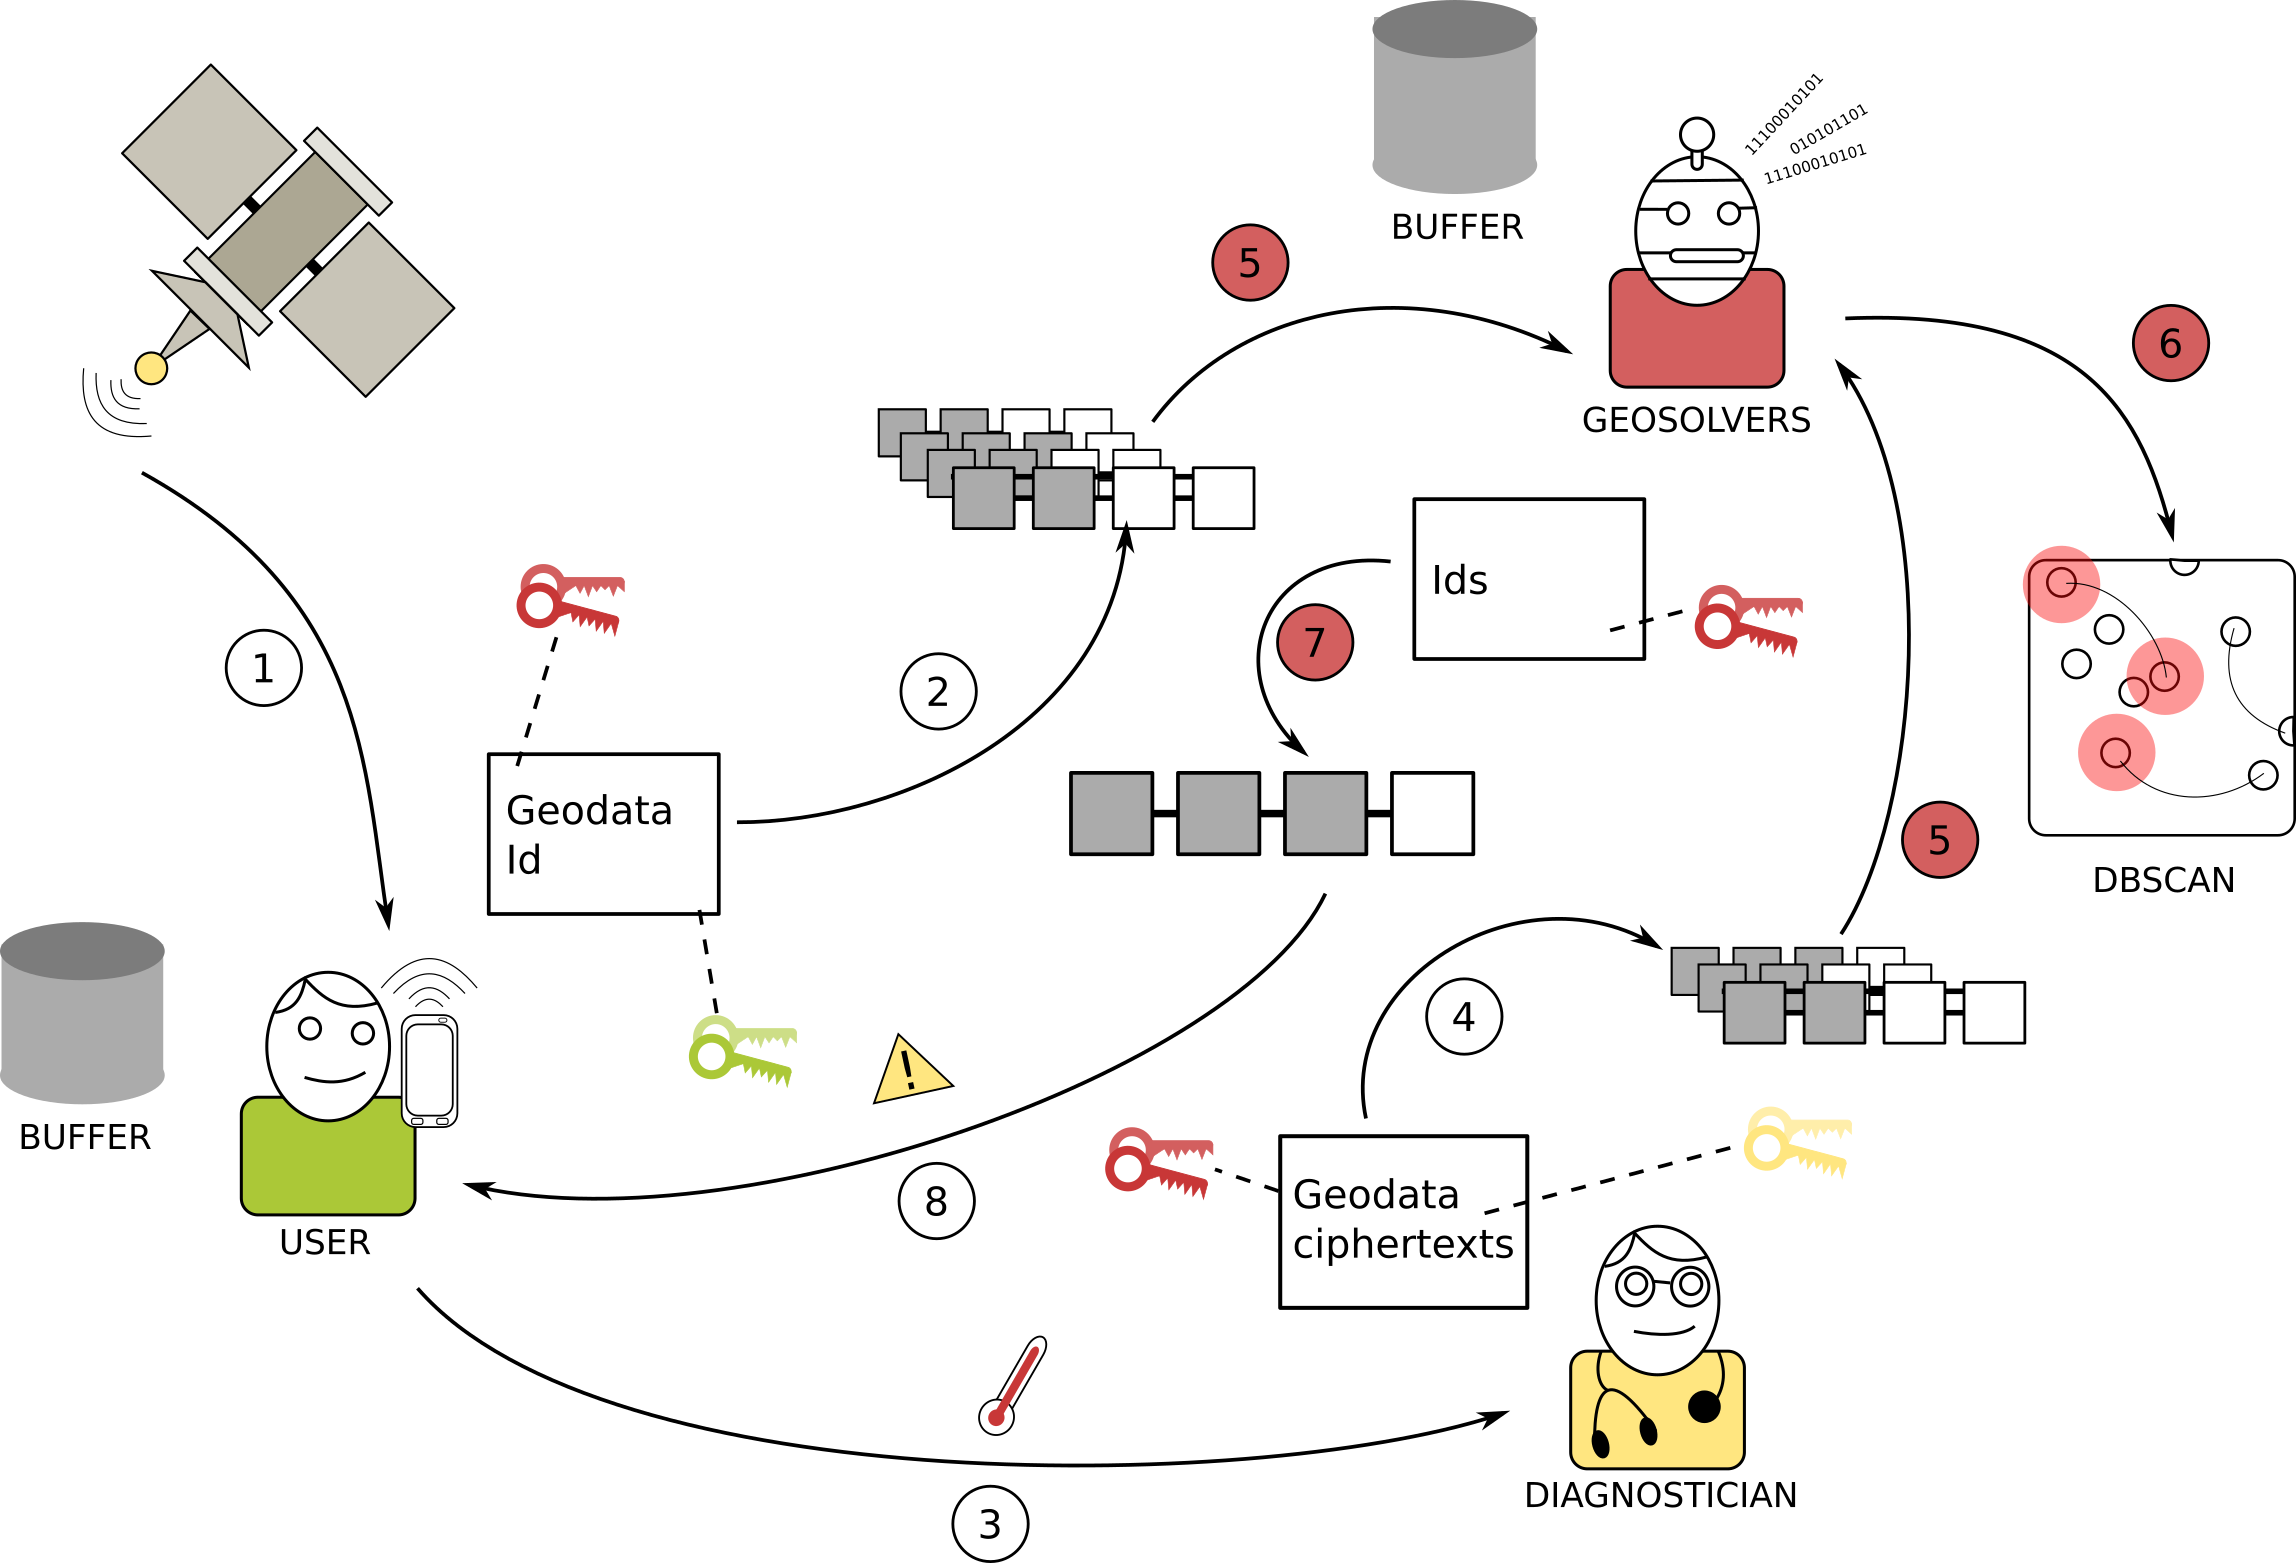
\includegraphics[width=0.95\linewidth]{images/design_geosolver.png}
\end{frame}

\begin{frame}{GeoSolver}
    \begin{block}{Characteristics}
        \begin{itemize}
            \item \textbf{Server} that is responsible for the computation of possible infected individuals
            \item Owns its personal \textbf{MAM channel}, which has a publicly known seed
            \item Owns a pair of \textbf{keys} to decrypt data from both agents and diagnosticians
            \item Owns a pair of \textbf{keys} to encrypt and sign its messages for all the agents
        \end{itemize}
    \end{block}
    
    \vspace{-3pt}
    
    \begin{block}{Infected Computation Procedure}
        Periodically, the geosolver fetches the new data added to the MAM channels of all the agents and all the diagnosticians, then it:
        \begin{itemize}
            \item [1.] Appends this data to its internal cache, and filters out transactions that are too old
            \item [2.] Runs a \textbf{DBSCAN} algorithm on the cached data to compute the IDs of the possible infected agents based on spatial and temporal proximity
            \item [3.] Encrypts this list of IDs using its private key and a public key which is paired to the shared key used by the agents
            \item [4.] Signs the obtained ciphertext with its private key
            \item [5.] Appends the ciphertext to its personal MAM channel, along with the signature
        \end{itemize}
    \end{block}
\end{frame}

\begin{frame}{GeoSolver}
    \begin{columns}
    \column{0.46\linewidth}
        \begin{block}{DBSCAN}
            \begin{itemize}
                \item \textbf{Clustering algorithm} like K-means
                \item \textbf{Density-based} rather than centroid-based
                \item Two hyperparameters:
                \begin{itemize}
                    \item[$\epsilon$] Distance
                    \item[$n$] Number of neighbors within that distance (1 in this case)
                \end{itemize}
            \end{itemize}
        \end{block}
        
        \vspace{5pt}
        
        \begin{block}{Clusters}
        \begin{itemize}
            \item All diagnosticians' transactions share the same fictional ID, representing an infected.
            \item Once clusters are computed by the algorithm, if in a cluster the aforementioned ID is present, all the members are notified.
        \end{itemize}
        \end{block}
        
    \column{0pt}
        
    \column{0.46\linewidth}
        \raggedleft
        \includegraphics[width = \linewidth]{images/dbscan.png}
    \end{columns}
\end{frame}